\section{Current Status Of Project}

This section describes the project as per the various stages of the Software Development life
cycle. The model of software development life cycle used in this project is the waterfall method.
The Waterfall Method is comprised of a series of very definite phases, each one run intended to
be started sequentially only after the last has been completed, with one or more tangible
deliverables produced at the end of each phase of the waterfall method of SDLC. Essentially, it
starts with a heavy, documented, requirements-planning phase that outlines all the requirements
for the project, followed by sequential phases of design, coding, test-casing, optional
documentation, verification (alpha-testing), validation (beta-testing), and finally
deployment/release.\\
\begin{figure}[H]
\centering 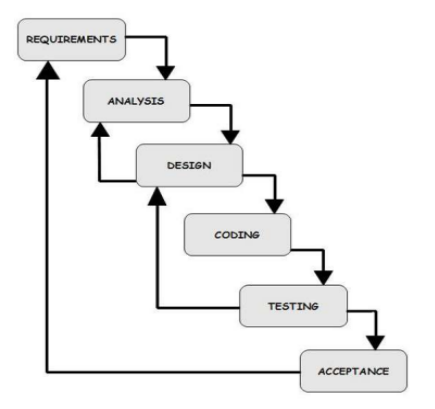
\includegraphics[scale=0.5]{image/sdlc.png}
\caption{Modified Waterfall Model}
\end{figure}

As shown in the Figure, the Waterfall model contains the following stages of software
development:
\begin{enumerate}
\item Requirement Analysis
\item Design
\item Implementation
\item Testing
\item Maintenance
\end{enumerate}
\begin{enumerate}
\item \textbf{\emph{Requirement Analysis:}}\\
Existing system is time consuming and it makes difficult to convey huge amount of users about
any event, class or seminar almost instantly. Also there is always a big crowd in front of
noticeboard. So it was hectic to read any useful instruction and information. Thus all the
problems of the existing system are summarized and proposing a new system that works as an
online application. It is a value added solution to the problem. It resolves all the problems stated
above. It will provide simple interface to the user to operate on and convey the intended users
about events almost instantly, anytime and anywhere.\\
Rests of the above stages of SDLC are under process.
\end{enumerate}
